\PassOptionsToPackage{unicode=true}{hyperref} % options for packages loaded elsewhere
\PassOptionsToPackage{hyphens}{url}
%
\documentclass[11pt,ignorenonframetext,]{beamer}
\usepackage{pgfpages}
\setbeamertemplate{caption}[numbered]
\setbeamertemplate{caption label separator}{: }
\setbeamercolor{caption name}{fg=normal text.fg}
\beamertemplatenavigationsymbolsempty
\usepackage{lmodern}
\usepackage{amssymb,amsmath}
\usepackage{ifxetex,ifluatex}
\usepackage{fixltx2e} % provides \textsubscript
\ifnum 0\ifxetex 1\fi\ifluatex 1\fi=0 % if pdftex
  \usepackage[T1]{fontenc}
  \usepackage[utf8]{inputenc}
  \usepackage{textcomp} % provides euro and other symbols
\else % if luatex or xelatex
  \usepackage{unicode-math}
  \defaultfontfeatures{Ligatures=TeX,Scale=MatchLowercase}
\fi
\usetheme[]{Montpellier}
\usecolortheme{beaver}
% use upquote if available, for straight quotes in verbatim environments
\IfFileExists{upquote.sty}{\usepackage{upquote}}{}
% use microtype if available
\IfFileExists{microtype.sty}{%
\usepackage[]{microtype}
\UseMicrotypeSet[protrusion]{basicmath} % disable protrusion for tt fonts
}{}
\IfFileExists{parskip.sty}{%
\usepackage{parskip}
}{% else
\setlength{\parindent}{0pt}
\setlength{\parskip}{6pt plus 2pt minus 1pt}
}
\usepackage{hyperref}
\hypersetup{
            pdftitle={Performances des modèles économétriques et de Machine Learning pour l'étude économique des choix discrets de consommation},
            pdfborder={0 0 0},
            breaklinks=true}
\urlstyle{same}  % don't use monospace font for urls
\newif\ifbibliography
% Prevent slide breaks in the middle of a paragraph:
\widowpenalties 1 10000
\raggedbottom
\setbeamertemplate{part page}{
\centering
\begin{beamercolorbox}[sep=16pt,center]{part title}
  \usebeamerfont{part title}\insertpart\par
\end{beamercolorbox}
}
\setbeamertemplate{section page}{
\centering
\begin{beamercolorbox}[sep=12pt,center]{part title}
  \usebeamerfont{section title}\insertsection\par
\end{beamercolorbox}
}
\setbeamertemplate{subsection page}{
\centering
\begin{beamercolorbox}[sep=8pt,center]{part title}
  \usebeamerfont{subsection title}\insertsubsection\par
\end{beamercolorbox}
}
\AtBeginPart{
  \frame{\partpage}
}
\AtBeginSection{
  \ifbibliography
  \else
    \frame{\sectionpage}
  \fi
}
\AtBeginSubsection{
  \frame{\subsectionpage}
}
\setlength{\emergencystretch}{3em}  % prevent overfull lines
\providecommand{\tightlist}{%
  \setlength{\itemsep}{0pt}\setlength{\parskip}{0pt}}
\setcounter{secnumdepth}{0}

% set default figure placement to htbp
\makeatletter
\def\fps@figure{htbp}
\makeatother

% Colors
% \usepackage{colortbl}

% Change section names style
\titlegraphic{
  \vspace{-30mm}
  \flushright
  %\includegraphics[height = 8mm]{../images/lig_logo_1.png}
  \includegraphics[height = 8mm]{../images/gael_logo_3.jpg}
  \includegraphics[height = 8mm]{../images/uga_logo.png} 
}

%%%%%%%%%%%%%%%%%
% Load Packages %
%%%%%%%%%%%%%%%%%

% Spacings
\usepackage{setspace}

% Tables
\usepackage{longtable}
\usepackage{tabu}

% Floats
\usepackage{morefloats}
\usepackage{float}
\usepackage{placeins}

% Highlighting
\usepackage{soul}

% Horizontal page position
\usepackage{pdflscape}

% Append pdfs
\usepackage{pdfpages}

% Add latex chunks
\usepackage{docmute}

% Short toc
\usepackage{shorttoc}
%\setcounter{tocdepth}{1}
%\usepackage{minitoc} - incompatible with document class

% Referencing mutliple things with a single command - \cref
\usepackage{cleveref}

% Array
\usepackage{array}
\usepackage{makecell}

% Multiple columns
\usepackage{multicol}

% Image insertion and colors
\usepackage{graphicx}

% Latex comments
\newenvironment{dummy}{}{}

% Fonts
% \usepackage{fontspec}
% \setmainfont{Museo}

% drawing
\usepackage{tikz}
\usetikzlibrary{matrix,chains,positioning,decorations.pathreplacing,arrows}

\usepackage{dcolumn}
% \usepackage{subfig}
\usepackage[export]{adjustbox}
% \usepackage[demo]{graphicx}  
\usepackage{subcaption}
\usetikzlibrary{shapes,arrows}
\usetikzlibrary{arrows.meta}
\usepackage[edges]{forest}

\usepackage{calc}
\usepackage{smartdiagram}

% Add footline
\makeatletter
\setbeamertemplate{footline}{%
  \leavevmode%
  \hbox{%
  \begin{beamercolorbox}[wd=.333333\paperwidth,ht=2.25ex,dp=1ex,center]{author in head/foot}%
    \usebeamerfont{author in head/foot}{Nikita Gusarov}
  \end{beamercolorbox}%
  \begin{beamercolorbox}[wd=.333333\paperwidth,ht=2.25ex,dp=1ex,center]{title in head/foot}%
    \usebeamerfont{institute in head/foot}\insertshortdate
  \end{beamercolorbox}%
  \begin{beamercolorbox}[wd=.333333\paperwidth,ht=2.25ex,dp=1ex,right]{date in head/foot}%
    \usebeamerfont{date in head/foot}\insertshortinstitute{}\hspace*{1em}
   %\insertframenumber{} / \inserttotalframenumber\hspace*{2ex} % old version
    \insertframenumber{} \hspace*{2ex} % new version without total frames
  \end{beamercolorbox}}%
  \vskip0pt%
}
\makeatother

\title{Performances des modèles économétriques et de Machine Learning pour
l'étude économique des choix discrets de consommation}
\providecommand{\subtitle}[1]{}
\subtitle{Projet Doctoral\\
\emph{Contribution méthodologique en économie et économétrie appliquée}}
\author{\large Nikita Gusarov\\
\small Master 2, MIASHS C2ES (UGA)\\
~\\
\raggedright\small Directeur de thèse:\\
\raggedright\hspace{10mm}\small Iragaël Joly, MCF HDR (GAEL, UGA,
Grenoble INP)\\
\raggedright\small Co-encadrant:\\
\raggedright\hspace{10mm}\small Pierre Lemaire, MCF (G-SCOP, Grenoble
INP)\\
\hspace{-20mm}}
\date{01/09/2020}

\begin{document}
\frame{\titlepage}

\hypertarget{introduction}{%
\section{Introduction}\label{introduction}}

\begin{frame}{Approche scientifique en économie \& économétrie}
\protect\hypertarget{approche-scientifique-en-economie-econometrie}{}

\begin{figure}
    \centering
    \label{fig:burel}
    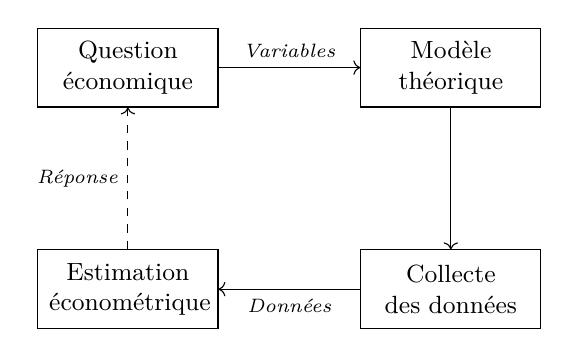
\begin{tikzpicture}[
        box/.style = {
            draw, 
            text width=2cm, 
            align=center, 
            minimum width={width("économétrique")+2pt},
            minimum height={1cm},
            font=\small
        },node distance=1.8cm]

        \node[box] (b) {Modèle\\théorique};
        \node[box, left=of b] (a) {Question\\économique};
        \node[box, below=of b] (c) {Collecte\\des données};
        \node[box, below=of a] (d) {Estimation\\économétrique};
        
        \draw[->] (a) -- (b) node[midway, above] {\textit{\scriptsize Variables}};
        \draw[->] (b) -- (c);
        \draw[->] (c) -- (d) node[midway, below] {\textit{\scriptsize Données}};
        \draw[dashed, ->] (d) -- (a) node[midway, left] {\textit{\scriptsize Réponse}};
    \end{tikzpicture}
\end{figure}

(Hensher, Rose, and Greene 2015)

\end{frame}

\begin{frame}{Exemple}
\protect\hypertarget{exemple}{}

Michaud, Llerena, and Joly (2012) étudient \textbf{les consentements à
payer pour les attributs environnementaux des produits non-alimentaires}
(\emph{des roses rouges})

\begin{figure}
    \centering
    \label{fig:burel}
    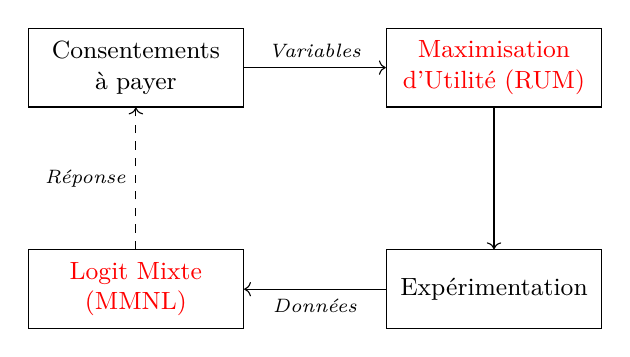
\begin{tikzpicture}[
        box/.style = {
            draw, 
            text width=2.5cm, 
            align=center, 
            minimum width={width("Expérimentation")+4pt},
            minimum height={1cm},
            font=\small
        },node distance=1.8cm]

        \node[box] (b) {\textcolor{red}{Maximisation d'Utilité (RUM)}};
        \node[box, left=of b] (a) {Consentements\\à payer};
        \node[box, below=of b] (c) {Expérimentation};
        \node[box, below=of a] (d) {\textcolor{red}{Logit Mixte (MMNL)}};
        
        \draw[->] (a) -- (b) node[midway, above] {\textit{\scriptsize Variables}};
        \draw[->] (b) -- (c);
        \draw[->] (c) -- (d) node[midway, below] {\textit{\scriptsize Données}};
        \draw[dashed, ->] (d) -- (a) node[midway, left] {\textit{\scriptsize Réponse}};
    \end{tikzpicture}
\end{figure}

\end{frame}

\begin{frame}{Mise en perspective - Revue de Littérature}
\protect\hypertarget{mise-en-perspective---revue-de-litterature}{}

\begin{itemize}
\tightlist
\item
  Questions sur l'\textbf{outil}

  \begin{itemize}
  \tightlist
  \item
    Performances comparées des \textcolor{red}{modèles de l'IA et du ML}
    avec les \textcolor{red}{modèles économétriques} traditionnels
    (Mihalovic 2016)?
  \end{itemize}
\item
  Questions sur l'\textbf{usage} de l'outil

  \begin{itemize}
  \tightlist
  \item
    Quelle taille d'\textcolor{red}{échantillon} choisir pour une
    puissance statistique donnée (Ye and Lord 2014)?
  \item
    Quelle \textcolor{red}{structure} de la base des données? Quelle
    méthode de \textcolor{red}{collecte des données} (Mannering and Bhat
    2014)?
  \end{itemize}
\item
  Questions d'\textbf{intégration} de l'outil dans l'\textbf{approche
  économique}

  \begin{itemize}
  \tightlist
  \item
    Quelle \textcolor{red}{validité externe} des résultats (Horváthová
    and Mokrišová 2020)?
  \item
    Les modèles de \textcolor{red}{machine learning} peuvent-ils être
    adaptés pour traiter des questions économiques (Varian 2014)
  \end{itemize}
\end{itemize}

\end{frame}

\begin{frame}{Objectif}
\protect\hypertarget{objectif}{}

\textbf{Question de recherche}:

\begin{center}
\Large 
\textit{L'étude économique des \textcolor{red}{choix discrets de consommation} à travers la \textcolor{red}{comparaison de performance des modèles} économétriques et des outils de l'IA et du ML}
\normalsize
\end{center}

\end{frame}

\hypertarget{methodologie}{%
\section{Méthodologie}\label{methodologie}}

\begin{frame}{Le \emph{framework} proposé}
\protect\hypertarget{le-framework-propose}{}

\begin{figure}
    \centering
    \label{fig:burel}
    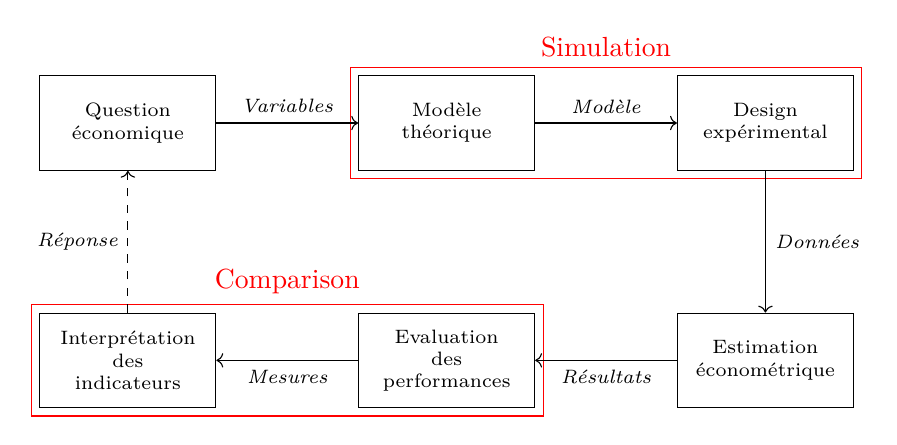
\begin{tikzpicture}[
        box/.style = {
            draw, 
            text width=2cm, 
            align=center, 
            minimum width={width("Interpretation")+2pt},
            minimum height={1.2cm},
            font=\scriptsize
        },node distance=1.8cm]

        \node[box] (b) {Modèle\\théorique};
        \node[box, left=of b] (a) {Question\\économique};
        \node[box, right=of b] (c) {Design\\expérimental};
        \node[box, below=of c] (d) {Estimation\\économétrique};
        \node[box, below=of b] (e) {Evaluation\\des\\performances};
        \node[box, below=of a] (f) {Interprétation\\des\\indicateurs};

        \node[rectangle, draw=red, fit=(b) (c), inner sep=1mm, label=above:{\textcolor{red}{Simulation}}] (bc) {};
        \node[rectangle, draw=red, fit=(e) (f), inner sep=1mm, label=above:{\textcolor{red}{Comparison}}] (ef) {};
        
        \draw[->] (a) -- (b) node[midway, above] {\textit{\scriptsize Variables}};
        \draw[->] (b) -- (c) node[midway, above] {\textit{\scriptsize Modèle}};
        \draw[->] (c) -- (d) node[midway, right] {\textit{\scriptsize Données}};
        \draw[->] (d) -- (e) node[midway, below] {\textit{\scriptsize Résultats}};
        \draw[->] (e) -- (f) node[midway, below] {\textit{\scriptsize Mesures}};
        \draw[dashed, ->] (f) -- (a) node[midway, left] {\textit{\scriptsize Réponse}};
    \end{tikzpicture}
\end{figure}

\end{frame}

\begin{frame}{Travail antérieur - Master 2}
\protect\hypertarget{travail-anterieur---master-2}{}

\textbf{Question étudiée:}

\begin{center}
Performances de modèles économétriques \textcolor{red}{multinomiaux} comparés au \textcolor{red}{réseau de neurones} en présence de \textcolor{red}{préférences hétérogènes} des consommateurs ?
\end{center}

\end{frame}

\begin{frame}{Travail antérieur - Master 2}
\protect\hypertarget{travail-anterieur---master-2-1}{}

\begin{itemize}
\tightlist
\item
  Un \emph{framework} permettant de
  \textcolor{red}{tester les hypothèses et théories}

  \begin{itemize}
  \tightlist
  \item
    \textcolor{red}{Deux} jeux des données artificielles :
    \newline préférences \textcolor{red}{hétérogènes} vs.
    \textcolor{red}{homogènes}
  \item
    \textcolor{red}{Trois} modèles issus de l'\emph{économétrie} et du
    \emph{machine learning}

    \begin{itemize}
    \tightlist
    \item
      Logit multinomial et Logit mixte
    \item
      Réseau de Neurones Convolutif
    \end{itemize}
  \end{itemize}
\item
  Evaluation des \textcolor{red}{performances} des modèles

  \begin{itemize}
  \tightlist
  \item
    Production des indicateurs économiques
  \item
    Précision

    \begin{itemize}
    \tightlist
    \item
      Prédiction
    \item
      Ajustement
    \end{itemize}
  \item
    Efficience en ressources
  \end{itemize}
\item
  \textcolor{red}{Une grille d'analyse} opérationelle
\end{itemize}

\end{frame}

\begin{frame}{Un framework adapté pour étudier:}
\protect\hypertarget{un-framework-adapte-pour-etudier}{}

\begin{block}{Structure des règles de décision de consommation}

\begin{itemize}
\tightlist
\item
  Comment les \textcolor{red}{régles de décision} affectent les
  estimations?

  \begin{itemize}
  \tightlist
  \item
    \emph{Random Utility Maximisation} (RUM)
  \item
    \emph{Random Regret Minimisation} (RRM)
  \item
    \emph{Quantum Decision Theory} (QDT)
  \end{itemize}
\item
  Comment les modèles se comportent face à différentes
  \textcolor{red}{structures des préférences}?

  \begin{itemize}
  \tightlist
  \item
    Hypothèse d'Indépendance aux Alternatives non Pertinentes (IIA) vs
    dépendance à l'alternative de référence
  \item
    Hypothèse d'utilité additive vs multiplicative
  \end{itemize}
\end{itemize}

Est-ce que les modèles de \emph{machine learning} sont compatibles avec
la \textcolor{red}{microéconomie}?

\end{block}

\end{frame}

\begin{frame}{Un framework adapté pour étudier:}
\protect\hypertarget{un-framework-adapte-pour-etudier-1}{}

\begin{block}{Spécification des préférences}

\begin{itemize}
\tightlist
\item
  Niveau de l'\textcolor{red}{individu}

  \begin{itemize}
  \tightlist
  \item
    Aversion au risque
  \item
    Transitivité des préférences
  \item
    \emph{autres apports de la behavioral economics}
  \end{itemize}
\item
  Niveau de la \textcolor{red}{population}

  \begin{itemize}
  \tightlist
  \item
    Hétérogénéité des préférences
  \item
    Hétérogénéité des règles de décision \& niveaux de rationnalité
  \end{itemize}
\end{itemize}

\end{block}

\begin{block}{Opportunité}

\begin{itemize}
\tightlist
\item
  Confronter \& rechercher les \textcolor{red}{complémentarités} entre

  \begin{itemize}
  \tightlist
  \item
    Données de \textbf{simulation} et données de
    l'\textbf{expérimentation}
  \item
    Outils du \textbf{ML} et modèles \textbf{économétriques}
  \end{itemize}
\end{itemize}

\end{block}

\end{frame}

\begin{frame}{Contributions de la thèse}
\protect\hypertarget{contributions-de-la-these}{}

\begin{itemize}
\tightlist
\item
  Un \textcolor{red}{outil d'aide à la conception} des études
  économiques et aux expérimentations
\item
  \textcolor{red}{Publications}

  \begin{itemize}
  \tightlist
  \item
    Etude des performances en présence des préférences hétérogènes à
    \emph{DA2PL} à Trento le 5-6 novembre 2020
  \item
    2 autres \emph{working-papers}, par ex.:

    \begin{itemize}
    \tightlist
    \item
      RUM vs RRM
    \item
      Simulation et expérimentation
    \end{itemize}
  \end{itemize}
\item
  Un \textcolor{red}{package \textit{R}} permettant de simuler des
  données de choix de consommation selon différents modèles
  comportementaux paramétrables
\end{itemize}

\end{frame}

\hypertarget{organisation}{%
\section{Organisation}\label{organisation}}

\begin{frame}{Collaboration et \emph{reproducible research}}
\protect\hypertarget{collaboration-et-reproducible-research}{}

\begin{figure}
    \centering
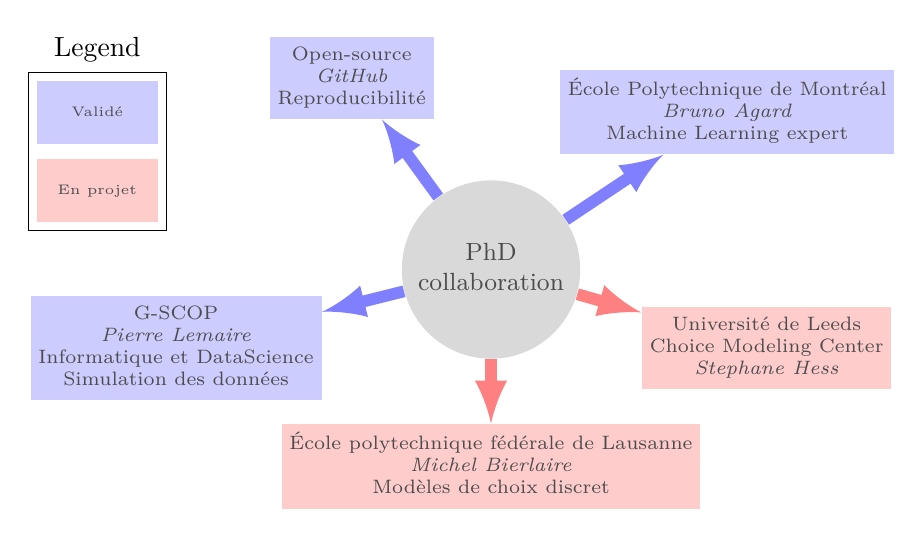
\begin{tikzpicture}
\tikzset{
    sun/.style={
        circle,
        color = black!70,
        fill = black!15,
        minimum size = 1cm,
        font = \small,
        inner sep = 0.1cm
    }
}
\tikzset{
    satellite/.style={
        rectangle,
        color = black!70,
        font = \scriptsize,
        minimum size = 1cm,
        inner sep = 0.1cm
    }
}
\tikzset{
    legend/.style={
        rectangle,
        color = black!70,
        font = \tiny,
        minimum size = 1cm,
        inner sep = 0.1cm,
        minimum width={width("En projet")+2pt},
        minimum height={0.8cm}
    }
}
\tikzset{
    satellitearrow/.style={
        -latex,
        line width = 0.15cm
    }
}

\draw (0,0) node (frame) [shape=regular polygon, regular polygon sides=5, minimum size=6cm, rotate=-36] {};

\node (sun) at (frame.center) [sun] {\makecell{PhD\\collaboration}};

\node (satellitea)  at (3,2) [satellite, fill=blue!20] 
    {\makecell{École Polytechnique de Montréal\\\textit{Bruno Agard}\\Machine Learning expert}};
\node (satelliteb)  at (-4, -1) [satellite, fill=blue!20] 
    {\makecell{G-SCOP\\\textit{Pierre Lemaire}\\Informatique et DataScience\\Simulation des données}};
\node (satellitec)  at (frame.corner 2) [satellite, fill=blue!20] 
    {\makecell{Open-source\\\textit{GitHub}\\Reproducibilité}};

\node (satellited)  at (0, -2.5) [satellite, fill=red!20] 
    {\makecell{École polytechnique fédérale de Lausanne\\\textit{Michel Bierlaire}\\Modèles de choix discret}};
\node (satellitee)  at (3.5, -1) [satellite, fill=red!20] 
    {\makecell{Université de Leeds\\Choice Modeling Center\\\textit{Stephane Hess}}};

\node (leg1) at (-5, 2) [legend, fill=blue!20] {Validé};
\node (leg2) at (-5, 1) [legend, fill=red!20] {En projet}; 
\node[rectangle, draw=black, fit=(leg1) (leg2), inner sep=1mm, label=above:{Legend}] (leg1leg2) {};

\draw [satellitearrow, draw=blue!50]  (sun) -- (satellitea);
\draw [satellitearrow, draw=blue!50]    (sun) -- (satelliteb);
\draw [satellitearrow, draw=blue!50]   (sun) -- (satellitec);
\draw [satellitearrow, draw=red!50]     (sun) -- (satellited);
\draw [satellitearrow, draw=red!50]  (sun) -- (satellitee);
\end{tikzpicture}
\end{figure}

\end{frame}

\begin{frame}{Le plan de travail}
\protect\hypertarget{le-plan-de-travail}{}

\hspace{-5cm}

\begin{center}\includegraphics{jury_files/figure-beamer/ggplo2_output-1} \end{center}

\end{frame}

\hypertarget{merci-de-votre-attention}{%
\section{Merci de votre attention}\label{merci-de-votre-attention}}

\begin{frame}{Merci de votre attention}
\protect\hypertarget{merci-de-votre-attention-1}{}

\begin{center}
\textbf{\textit{Performances des modèles économétriques et de Machine Learning pour l'étude économique des choix discrets de consommation}}

Nikita Gusarov

\small Master 2
MIASHS C2ES (UGA)
\end{center}

\raggedright\small Directeur de thèse:

\raggedright\hspace{10mm}\small Iragaël Joly, MCF HDR (GAEL, UGA,
Grenoble INP)

\raggedright\small Co-encadrant:

\raggedright\hspace{10mm}\small Pierre Lemaire, MCF (G-SCOP, Grenoble
INP)

\end{frame}

\begin{frame}{Références}
\protect\hypertarget{references}{}

\tiny

\hypertarget{refs}{}
\leavevmode\hypertarget{ref-breiman2001stat}{}%
Breiman, Leo, and others. 2001. ``Statistical Modeling: The Two Cultures
(with Comments and a Rejoinder by the Author).'' \emph{Statistical
Science} 16 (3). Institute of Mathematical Statistics: 199--231.

\leavevmode\hypertarget{ref-hensher2015}{}%
Hensher, David A., John M. Rose, and William H. Greene. 2015.
\emph{Applied Choice Analysis}. 2nd ed. Cambridge University Press.
\url{https://doi.org/10.1017/CBO9781316136232}.

\leavevmode\hypertarget{ref-horvathova2020comparison}{}%
Horváthová, Jarmila, and Martina Mokrišová. 2020. ``Comparison of the
Results of a Data Envelopment Analysis Model and Logit Model in
Assessing Business Financial Health.'' \emph{Information} 11 (3).
Multidisciplinary Digital Publishing Institute: 160.

\leavevmode\hypertarget{ref-mannering2014analytic}{}%
Mannering, Fred L, and Chandra R Bhat. 2014. ``Analytic Methods in
Accident Research: Methodological Frontier and Future Directions.''
\emph{Analytic Methods in Accident Research} 1. Elsevier: 1--22.

\leavevmode\hypertarget{ref-llerena2013rose}{}%
Michaud, Celine, Daniel Llerena, and Iragael Joly. 2012. ``Willingness
to pay for environmental attributes of non-food agricultural products: a
real choice experiment.'' \emph{European Review of Agricultural
Economics} 40 (2): 313--29. \url{https://doi.org/10.1093/erae/jbs025}.

\leavevmode\hypertarget{ref-mihalovic2016performance}{}%
Mihalovic, Matús. 2016. ``Performance Comparison of Multiple
Discriminant Analysis and Logit Models in Bankruptcy Prediction.''
\emph{Economics \& Sociology} 9 (4). Centre of Sociological Research
(NGO): 101.

\leavevmode\hypertarget{ref-varian2014bd}{}%
Varian, Hal R. 2014. ``Big Data: New Tricks for Econometrics.''
\emph{Journal of Economic Perspectives} 28 (2): 3--28.
\url{https://doi.org/10.1257/jep.28.2.3}.

\leavevmode\hypertarget{ref-ye2014comparing}{}%
Ye, Fan, and Dominique Lord. 2014. ``Comparing Three Commonly Used Crash
Severity Models on Sample Size Requirements: Multinomial Logit, Ordered
Probit and Mixed Logit Models.'' \emph{Analytic Methods in Accident
Research} 1. Elsevier: 72--85.

\normalsize

\end{frame}

\hypertarget{annexes}{%
\section{Annexes}\label{annexes}}

\begin{frame}{Econometrics against ML (Breiman and others 2001)}
\protect\hypertarget{econometrics-against-ml-breiman2001stat}{}

\begin{figure}[hbtp]
\centering
\label{fig:parad}
\begin{subfigure}[c]{.4\linewidth}
    \centering
    \caption{Real world}
    \label{fig:parad1}
    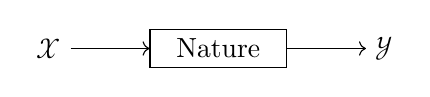
\begin{tikzpicture}[box/.style = {draw, text width=1.5cm, align=center}]
        \node[box] (b) {Nature};
        \node[left=of b] (a) {$\mathcal{X}$};
        \node[right=of b] (c) {$\mathcal{Y}$};
        \draw[->] (a) -- (b);
        \draw[->] (b) -- (c);
    \end{tikzpicture}
\end{subfigure}\vspace{12pt}

\begin{subfigure}[c]{.3\textwidth}
    \centering
    \caption{Econometrics}
    \label{fig:parad2}
    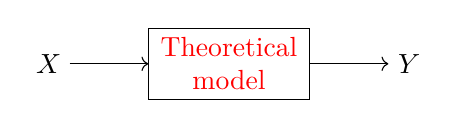
\begin{tikzpicture}[box/.style = {draw, text width=1.8cm, align=center}]
        \node[box] (b) {\textcolor{red}{Theoretical\\model}};
        \node[left=of b] (a) {$X$};
        \node[right=of b] (c) {$Y$};
        \draw[->] (a) -- (b);
        \draw[->] (b) -- (c);
    \end{tikzpicture}
\end{subfigure}
\hfill
\begin{subfigure}[c]{.3\linewidth}
    \centering
    \caption{Machine learning}
    \label{fig:parad3}
    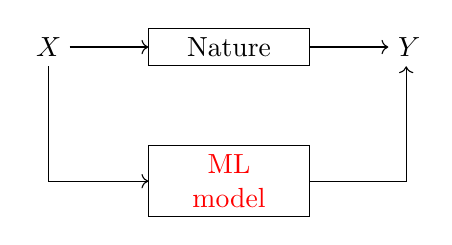
\begin{tikzpicture}[box/.style = {draw, text width=1.8cm, align=center}]
        \node[box] (b) {Nature};
        \node[box, below=of b] (d) {\textcolor{red}{ML\\model}};
        \node[left=of b] (a) {$X$};
        \node[right=of b] (c) {$Y$};
        \draw[->] (a) -- (b);
        \draw[->] (b) -- (c);
        \draw[->] (a) |- (d);
        \draw[->] (d) -| (c);
    \end{tikzpicture}
\end{subfigure}
\hspace{2cm}
\end{figure}

\end{frame}

\end{document}
